\documentclass{standalone}

\usepackage[OT1]{fontenc}
\renewcommand*\familydefault{\sfdefault}
\usepackage{helvet,sfmath}
\usepackage{siunitx}

\usepackage{tikz}
\usetikzlibrary{arrows,calc,patterns}
% \usetikzlibrary{intersections, calc, arrows.meta}
\usepackage{tikz,tkz-euclide}

\begin{document}
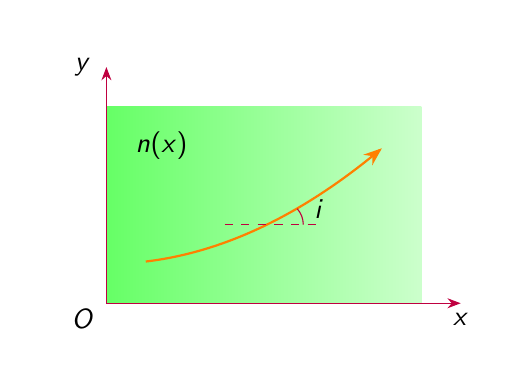
\begin{tikzpicture}[scale=1.0, >=Stealth]

    %% Background
    \draw[draw=none] (-1,-1) rectangle (5,3);

    % Gradient index
    \shade[left color = green!60, right color = green!20]
    (0,-0.5) rectangle (4,2);

    % Light
    \draw[thick, orange, domain=0.5:3.5, samples = 100, smooth, variable=\t, -Stealth] 
    plot ({\t}, {0.12*\t*\t});

    %Coordinate
    \draw[purple, -Stealth] (0,-0.5) to (4.5,-0.5);
    \draw[purple, -Stealth] (0,-0.5) to ( 0,2.5);

    \draw
    (-0.3,2.5) node{\(y\)}
    (4.5,-0.7) node{\(x\)}
    (-0.3,-0.7) node{\(O\)}
    ;

    % incident angle
    \draw[purple, dashed] (1.5,0.5) -- (2.7,0.5);
    \draw[purple] (2.5,0.5) arc (0:42:0.3);

    \draw
    (2.7,0.7) node{\(i\)}
    (0.7,1.5) node{\(n(x)\)}
    ;

\end{tikzpicture}
\end{document}